% Author	Rajath Shashidhara
% Email		rajath.shashidhara@gmail.com
%
% This work is licensed under the Creative Commons Attribution 4.0 International License. 
% To view a copy of this license, visit http://creativecommons.org/licenses/by/4.0/.

\chapter{AAH model with Oscillating Magnetic Field}
Driving in this model is introduced in the form of a rapidly oscillating magnetic field perpendicular to the 2D lattice plane. This is a notoriously hard
problem because as magnetic flux varies with time, the $q$-subband structure is no longer present. In fact, $q$ is an extremely discontinuous function of time and of course
it cannot be ascribed a closed form description. This variant of the AAH model was absent in scientific literature until our recent publication \cite{mishra2016phase}.
We deal with this problem using the time-independent effective Hamiltonian picture presented in Chapter \ref{ch:fl}.

\section{Effective Hamiltonian}
Magnetic vector potential $\mathbf{A}(t)$ (written in Landau gauge) is
\begin{equation}
 \mathbf{A}(t) = Bx \cos(\omega t) \hat{\mathbf{y}}
\end{equation} where $\omega$ is the driving frequency, and it is assumed to be very high.
The Hamiltonian in the tight-binding form is
\begin{equation}
 \hat{H} = \sum_{n} \ket{n}\bra{n+1} + \ket{n}\bra{n-1} + V_{0}\cos(2\pi\alpha_{0}n\cos(\omega t) + \theta)\ket{n}\bra{n}
\end{equation}

The effective Hamiltonian up to order $\mathcal{O}(\frac{1}{\omega^3})$ is
\begin{equation}
 \begin{split}
  \hat{H}_{eff} &= \sum_{n} \ket{n}\bra{n+1} + \ket{n}\bra{n-1} + V_{0}\cos(\theta)\sum_{n}\mathcal{J}_{0}(2\pi\alpha_0 n)\ket{n}\bra{n} \\
  &- \frac{1}{2\omega^2}V_{0}^2 \cos^{2}(\theta) \sum_{n}\sum_{j=1} (\mathcal{J}_{2j}(2\pi\alpha_0 (n+1)) - \mathcal{J}_{2j}(2\pi\alpha_0 n))^2 \ket{n}\bra{n+1} \\
  &- \frac{1}{2\omega^2}V_{0}^2 \sin^{2}(\theta) \sum_{n}\sum_{j=1} (\mathcal{J}_{2j-1}(2\pi\alpha_0 (n+1)) - \mathcal{J}_{2j-1}(2\pi\alpha_0 n))^2 \ket{n}\bra{n+1} \\ 
  & + h.c.
 \end{split}
\end{equation}
Effective Hamiltonian is found to have retained the tri-diagonal structure in position space.

\section{Metal-Insulator transition}
This model also displays a sharp metal-insulator transition like the AAH model. However, it is not self-dual. A detailed discussion can be found
in \cite{mishra2016phase}.

\begin{figure}[h]
 \caption{The metal-to-insulator transition of the Effective Hamiltonian for the system’s ground state.  Plots (c) and (d) are the real- and dual-space plots for the
ground state with phase $\theta = 0$.}
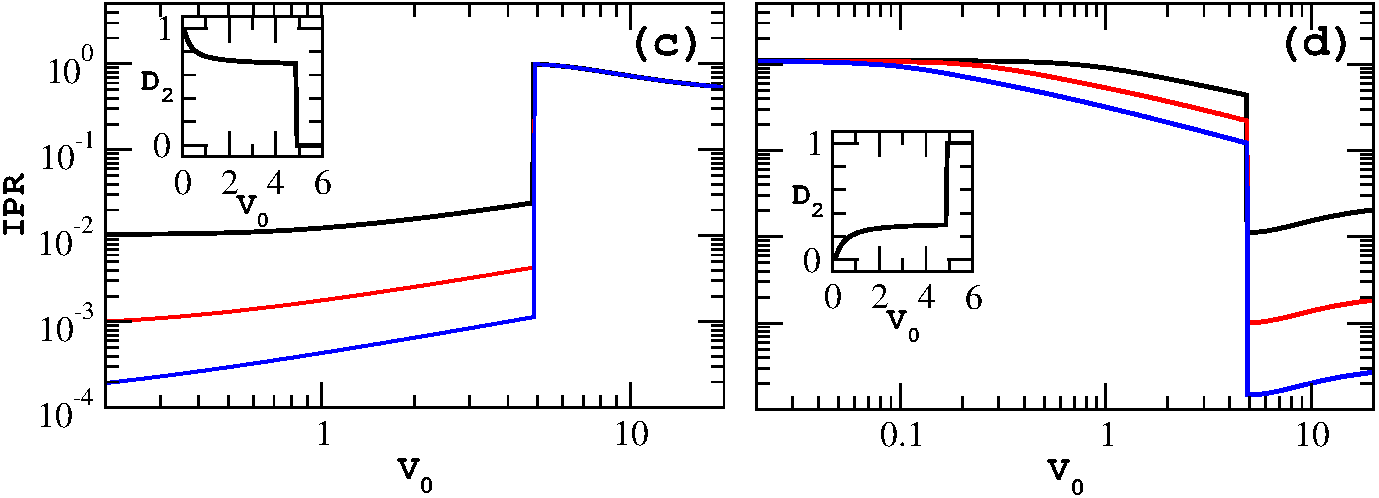
\includegraphics[width=0.85\textwidth]{FAA-Phase0-IPR-D2-Vs-V1byV2}
\centering
\end{figure}

\section{Spectrum}
The striking feature of the spectrum is the presence of energy-dependent mobility edge, an edge that splits the spectrum into two regions, one containing localized states and 
other containing delocalized states. This is a significant result as the mobility edge is atypical of 1-dimensional models \cite{mishra2016phase}.

\begin{figure}[ht]
\centering
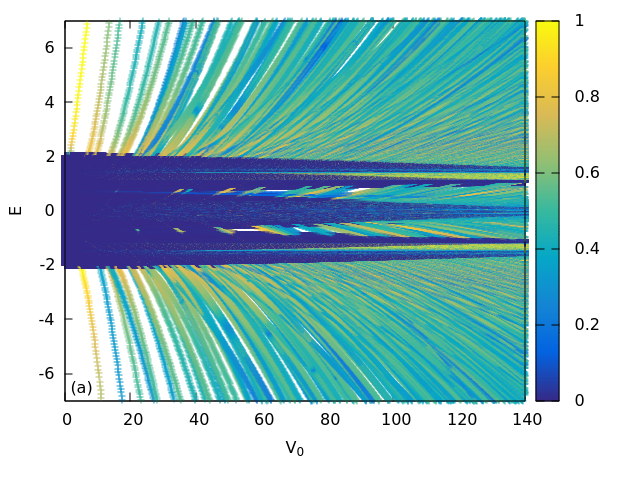
\includegraphics[width=0.65\textwidth]{evipr-4181-0.png}\\
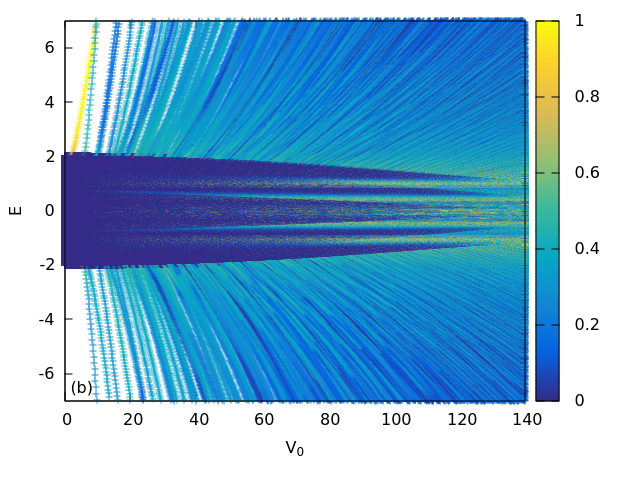
\includegraphics[width=0.65\textwidth]{evipr-4181-pi4.png}\\
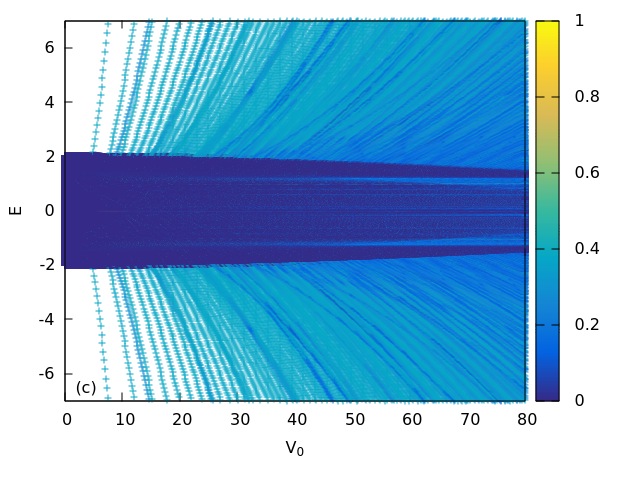
\includegraphics[width=0.65\textwidth]{evipr-4181-pi2.png}
\caption{The localization phase diagram with IPR in the (E,$V_0$) phase plane, for lattice size L = 4181 and three values of the variable $\theta$:
(a) $\theta = 0$, (b) $\theta = \pi/4$, (c) $\theta = \pi/2$}
\label{fig:mobedge}
\end{figure}

In order to qualitatively analyze some of our results we  consider a simplified model comprising of a trivial constant hopping term and an on-site potential $T$ which is aperiodic or quasi-periodic. The Schr\"odinger equation is given by  
\begin{equation}
\label{eq:AA}
 a_{n+1} + a_{n-1} + \Lambda  T(\alpha_0 n + \phi)a_n= Ea_n
\end{equation}
where,  $\Lambda$ is the strength of
on-site energy and $E$ are  the energy eigenvalues. One can go to the dual
space for the above system by defining an expansion, as follows
\begin{equation}
\label{trans1}
 a_n = \frac{ e^{ikn}}{\sqrt L}\displaystyle\sum_m \tilde{a}_m
 e^{i\,m(\alpha_0 n + \phi)}
\end{equation}
where, the $\tilde{a}_m$'s are the dual space amplitudes, and $k$ is a wave vector
from the Bloch wave expansion ansatz.  This  allows 
 $T$  to be expressed as
\begin{equation}
\label{trans2}
  T(\alpha_0 n+ \phi) = \frac{1}{\sqrt L}\displaystyle\sum_{\acute{m}}\mathcal{T}_{\acute{m}} e^{i\,\acute{m}(\alpha_0 n + \phi)}.
\end{equation}

Equations \eqref{trans1} and \eqref{trans2}  yield an on-site term in the dual space from the the hopping terms of Eq.\eqref{eq:AA} as  
\begin{equation}
\label{eq:Fspacesite}
a_{n-1} + a_{n+1} = \frac{e^{ikn}}{\sqrt L}\displaystyle\sum_m \tilde{a}_m e^{i\,m(\alpha_0 n + \phi)} \cos(\alpha_0 m + k)
\end{equation}
with a cosine modulation of the on-site energy  (as seen in
the Aubry and Andr\'e model). Interestingly, the real space on-site energy term transforms as
\begin{equation}
\Lambda  T(\alpha_0 n + \phi)a_n= \frac{\Lambda e^{ikn}}{L}\displaystyle\sum_{\acute{m}}\displaystyle\sum_m\mathcal{T}_{\acute{m}}\tilde{a}_m e^{i\,(m + \acute{m})(\alpha_0 n+\phi)}.   
\end{equation}
The RHS can be slightly rearranged to give 
\begin{equation}
\label{farTB}
\begin{split}
\frac{\Lambda e^{ikn}}{L}&\displaystyle\sum_{\acute{m}\neq\pm1}\displaystyle\sum_m\mathcal{T}_{\acute{m}}\tilde{a}_{m + \acute{m}} e^{i\,m(\alpha_0 n+\phi)} +\\ 
& \frac{\Lambda e^{ikn}}{L}\displaystyle\sum_m (\mathcal{T}_1\tilde{a}_{m-1} + \mathcal{T}_{-1}\tilde{a}_{m+1})e^{i\,m(\alpha_0 n + \phi)} 
\end{split}
\end{equation}
In the above form,  the second term clearly indicates the apparent nearest
neighbor hopping terms in the dual space whose strength is modulated
by the Fourier components of $T$. It is the first term in the above
expression which explicitly breaks the exact duality. The form of
$\mathcal{T}_{\acute{m}}$ determines the extent to which different
$m$ values in the dual space are coupled.  It is well known
that for decaying oscillatory functions like Sinc and Bessel function
of the zeroth order $\mathcal{T}_{\acute{m}}$ is a rectangular
function,   with possibly a $\acute{m}$ dependent modulation,  symmetric
about the origin. Thus,  in our case, we expect a truncation effect in
dual space which restricts the range of couplings. This deviation from
exact duality is expected to have some impact on the
probability of an ``analytic accident'' along the lines of \parencite{aubry1980analyticity}.
The appearance of localized states (real eigenfunctions) happens when
there are superpositions of counter-propagating plane waves with
wave vectors of near-commensurate magnitude. This would mean,  in our
model, some harmonics from the expansion of $T$ shall scatter the wave with
wave vector $k$ by an amount commensurate with $2n\pi$. This has to be
considered together with the fact that for a rational approximation of
$\alpha_0$ as a ratio of two large successive Fibonacci numbers, the
true momentum(Fourier) space eigenvalues $\kappa$ are related to $m$
as $ \kappa = mF_{i-1}\textrm{mod}F_i$, where $F_{i-1}$ and $F_i$ are
successive Fibonacci numbers \parencite{kohmoto1983metal,aulbach2004phase}. Thus, what appear
to be close neighbors in $m$ could possibly be well separated in the
actual wave vector space. Further, the range of $m$ values that shall
remain coupled in the dual space will be dictated by the extent of
$T$ in the real lattice for example the first zero in the Bessel
function. The set of $m$'s which conspires with a given $k$ value to
yield a localized state shall be dictated by $V_0$ and $E(k)$. This
explains the energy dependent mobility edge in Fig.\ref{fig:mobedge}. 

In the dual space, where $k$ acts as a phase (see Eq.\eqref{eq:Fspacesite}), a
state localized at few $m$ values could be  shifted by large amounts
for a small change in $k$. This allows for the interpretation that a
small change in $\phi$ could in effect cause a state localized around
some lattice site to localize about a far off site.
 In terms of symmetry, the absence of 
translational invariance in Euclidean space of quasi-periodic
structures with two incommensurate periodicities can be restored in an
extended space using the $\phi$ dimension \cite{sokoloff1985unusual, janner1977symmetry}. This
effect of $\phi$ on localization properties leads to the differences between the
three plots in Fig.\ref{fig:mobedge}.  
